% Class for the academic internship paper :
\documentclass[utf8,final]{stageM2R}

\usepackage{graphicx}
\usepackage{float}
\usepackage[french]{babel}

\usepackage[draft]{commands} % Custom commands, defined in this folder

\supervisors{Noura \textsc{Faraj}\\Christophe \textsc{Fiorio}\\Benjamin \textsc{Charlier}}
\location{LIRMM UM5506 - CNRS, Université de Montpellier}
\title{Gestion, traitement et visualisation d'images médicales à très haute résolution}
\track{IMAGINA}
\date{2 Juillet 2020}
\version{6}
\author{Thibault}

\abstractfr{}
%\abstracten{}

\begin{document}
	\selectlanguage{french}
	\frontmatter \maketitle
	\cleardoublepage
	\tableofcontents \mainmatter

	\commentaire{\raggedright
		Plan proposé pour l'instant :\\
		\begin{enumerate}
			\item Introduction au stage, et aux problématiques
			\item Continuation de l'état de l'art, introduction poussée au domaine
			\item Travail réalisé sur le stage
			\item Travail réalisé sur le papier avec Noura
			\item Travail à venir -- Thèse ! (si conclusion, parler de thèse dans conclusion, pas ici)
			\item Conclusion (?) -- peut être a mettre avec (5)
		\end{enumerate}
	}

	% Chapitre 1 : Introduction
\chapter{Introduction}\label{chapter:01:introduction}
{
    \section{Diagnostics du cancer de la prostate}\label{section:contexte} % "par coupes histologies" en plus ?
    {
        \emph{Ce stage, financé par le LabEx NUMEV, s'inscrit dans le cadre d'une collaboration internationale entre l'université de Tulane dans la ville de Nouvelle Orléans, et l'université de Montpellier sur un projet d'aide à la détection du cancer de la prostate.}\medskip

        Le cancer de la prostate est aujourd'hui diagnostiqué grâce à l'échelle de Gleason (décrite à la section \ref{section:gleason_scale}) qui représente les contours des glandes de la prostate à différent stade de la maladie. L'échelle de Gleason est construite à partir de coupes histologiques\definition{Coupes effectuées dans un tissu biologique} planaires et comporte des croquis de chaque type de glandes. Cette méthode de diagnostic présente une grande variabilité selon l'opérateur (figure \ref{img:gleason_bias}). Ces différences dans le diagnostic peuvent être expliquées par deux facteurs: la variance de la forme des glandes engendrée par le choix de l'orientation des plans de coupe dans le tissu, mais aussi par le manque de précision des dessins servant de référence dans l'échelle de Gleason (figure \ref{img:gleason_scale}). Afin d'améliorer le diagnostic du cancer de la prostate, il apparaît nécessaire de développer de nouvelles techniques de détection de structures cancéreuses. L'approche envisagée ici est l'étude tridimensionnelle de la forme des glandes dans un échantillon de prostate, permettant ainsi d'éliminer la variabilité due à l'angle de coupe dans la méthode de Gleason. Nos collaborateurs de l'université de Tulane à la Nouvelle Orléans ont pour cela développé un microscope à feuillet de lumière permettant de capturer une image 3D d'un échantillon de tissu humain (voir la section \ref{section:microscopy}). Une reconstruction volumique d'un échantillon de prostate permettra une étude morphologique et topologique des glandes afin d'enrichir les méthodes de diagnostic du cancer.

        \begin{figure}[h]
            \centering
            \includegraphics[width=.7\linewidth]{img/gleason_bias.png}
            \captionsetup{width=.8\linewidth, labelfont=bf}
            \caption{Variabilité inter-opérateur pour les diagnostics de l'échelle de Gleason d'un même échantillon.\cite{cite_gleason_bias}}
            \label{img:gleason_bias}
        \end{figure}
        
        Le microscope créé par les chercheurs de l'université de Tulane est extrêmement précis, générant des images dont la résolution spatiale est inférieure au micromètre. Leur technique d'acquisition (voir section \ref{section:microscopy} pour plus d'informations) nécessite l'utilisation de deux capteurs en tandem effectuant des vues par coupe de l'échantillon. Cela génère, pour une seule acquisition, deux piles d'images correspondant à des points de vue différents. Ces deux piles d'images doivent donc être fusionnées de manière cohérente pour reconstruire la structure 3D et visualiser l'échantillon. Mais la taille des images, ainsi le nombre de prises de vues, rend impossible le stockage en mémoire vive d'une acquisition. Cela rend l'analyse de l'échantillon particulièrement complexe.
        }
        
\section{Objectif du stage: Vers une modélisation 3D des glandes de la prostate}\label{section:contrib}
    {
        L'objectif de ce stage est de proposer un système de visualisation interactive des données, permettant une première exploration de la forme des glandes. Notre travail comporte deux axes principaux. Le premier axe présente plusieurs méthodes de visualisation permettant d'afficher un jeu de données massif: une exploration par plans de coupes ou une visualisation volumique par sous-domaine. %Afin d'atteindre cet objectif, une prise en main des outils de développement sera nécessaire, pour se familiariser avec les jeux de données. Ensuite, il nous faudra établir une méthode permettant la gestion des données, afin de pouvoir les afficher à l'écran, et les manipuler en temps réel.
        Les données ne pouvant pas rentrer en mémoire sur des stations de travail standard, une première méthode de pré-traitement pour la visualisation sera mise en place, ne chargeant qu'une version basse résolution des images. Pour finir, nous proposerons deux méthodes de visualisations pour les jeux de données. Une première méthode permettra une exploration interactive des jeux de données chargés en mémoire par l'utilisation de plans de coupe. Ensuite, une autre méthode de visualisation par sous-domaine sera présentée. Cette méthode fut originellement développée pour visualiser des images segmentées, mais peut être adaptée pour visualiser des images non-segmentées. Les travaux réalisés sur la méthode de visualisation par sous-domaines ont fait l'objet d'une soumission à la conférence IEEE VIS 2020, en collaboration avec Mme \textsc{Faraj} ainsi que M.\textsc{Summa}.

        Par la suite, il nous faudra proposer une méthode reconstruisant les deux piles présentes dans le jeu de données en une seule image médicale, en tenant compte des différentes caractéristiques des prises de vues. Pour ce faire, il faudra proposer une méthode de reconstruction prenant en compte les conditions de prises de vues particulières des piles d'images stockées en mémoire. Nous commencerons par proposer une méthode de recherche de voisins en espace affine, et continuerons sur une méthode de génération de grille prenant en compte cette recherche de voisins, afin de créer des grilles de résolution et de taille arbitraire. Afin de réduire l'empreinte mémoire, ces deux méthodes sont réalisées à la volée pour permettre le traitement d'une plus grande quantité de données.

        \iffalse
        \noindent\commentaire{Nouveau plan suggéré (majoritairement réorganisation, pas de contenu en +) :\begin{itemize}
            \item Intro
            \item partie 'prise en main' :\begin{itemize}
                \item chargement des données\begin{itemize}
                    \item présentation méthode de stockage mémoire (section 2.1 maintenant)
                    \item présentation interpolation
                \end{itemize}
                \item visu par plans de coupe (même texte)
                \item visu par sous-domaines (même texte)
            \end{itemize}
            \item partie travail de stage :\begin{itemize}
                \item présentation du problème (présentation des différents espaces depuis fig 4.1 principalement, plus présentation dual-visu en adéquation avec le problème)
                \item recherche de voisins\begin{itemize}
                    \item méthodes d'interpolation (comparaison, à faire après résultats)
                    \item implémentation
                    \item résultats (ici, ou plutot dans résultats génération grille ?)
                \end{itemize}
                \item reconstruction de grilles\begin{itemize}
                    \item méthode utilisée
                    \item implémentation
                    \item tests
                    \item résultats (à venir)
                \end{itemize}
            \end{itemize}
            \item conclusion
        \end{itemize}}
        \fi
    }
    
        
	% }}}

}
% VIM modeline : do not touch !
% vim: set spell spelllang=fr :


	% Chapitre 02 : Etat de l'art
\chapter{État de l'art}\label{chapter:02:stateoftheart}
{
	\commentaire{
		A parler :~\begin{enumerate}
			\item représentations volumiques (voxels, intérêt dans scans médicaux)
			\item reconstructions volumiques (remeshing, interpolations ...)
			\item Gleason, prostate en général
			\item Méthodes de microscopie : LSM, SPIM, di-SPIM (overview des 3)
			\item implémentation spécifique à Tulane
			\item présentation rapide pour transition des travaux ajoutés qu'on va faire
		\end{enumerate}
	}\par

	% section volume {{{
	\section{Représentations volumiques}
	{
		Le but de ce projet étant d'analyser la morphologie des glandes de la prostate d'un patient, il nous est nécessaire d'avoir une façon de représenter cette morphologie en trois dimensions. Une première approche pourrait être de représenter uniquement les surfaces de contact entre différents tissus et glandes dans l'échantillon analysé. Mais une telle méthode de reconstruction requiert beaucoup de traitement. Heureusement, il existe une autre façon de représenter un espace tridimensionnel : les grilles volumiques, aussi appelées grilles de voxels.\par

		% Grilles voxels {{{
		\subsection{Grilles de voxels}
		{
			\wip{Ajouter avantages, inconvénients : pour l'instant on a que une vue de la chose, sans rapport au stage}\\

			Tout comme le son et la photographie, une grille grille volumique, est une représentation $n$-dimensionnelle d'un signal. Dans le cas du son, ce signal est unidimensionnel, car l'information qu'il contient ne varie que sur une seule dimension temporelle. Une photographie varie selon deux dimensions spatiales. Une grille volumique, quand à elle, varie selon trois dimensions spatiales. Elle est la représentation discrète d'une fonction implicite tridimensionnelle continue attribuant une valeur, que ce soit une couleur, une température, ou une quelconque autre propriété à chaque point de l'espace. Chacun de ses éléments sont appelés voxels, pour \textit{\textbf{Vo}}\textit{lumetric} \textit{\textbf{El}}\textit{ement}, de la même façon que un élément d'une image est appelé pixel, pour \textit{\textbf{Pi}}\textit{cture} \textbf{\textit{El}}\textit{ement}.\par

			Ces grilles volumiques, aussi appelées grilles de voxels, sont très utiles pour représenter la discrétisation d'une fonction dans l'espace. Ces grilles de voxels commencent à être utilisées dans le domaine du public depuis quelques années, dans des jeux tels que Minecraft, ou encore dans certains moteurs de rendu pour mieux représenter un milieu participant comme un nuage de fumée par exemple. Malgré cela, leur premières utilisations furent dans le domaine médical. En effet, il est trivial de reconstruire une grille de voxels à partir d'un ensemble d'images transversales d'un volume. Par exemple, le projet Visible Human\footnote{Voir \protect{\url{https://www.nlm.nih.gov/research/visible/visible_human.html}}~}~\cite{cite_visible_human} permet d'obtenir un ensemble de coupes de haute résolution d'un corps humain. Il serait en facile de construire une grille de voxels à partir de ce jeu de données, afin d'obtenir une représentation tridimensionnelle du corps photographié.\par

			\commentaire{Mettre illustration de grille de voxels ici, ou de visible human}\par

			Il est toutefois important de noter que malgré le fait que les grilles de voxels sont techniquement une structure de partitionnement de l'espace tridimensionnel, elles ne sont pas optimisées pour partitionner efficacement l'espace au niveau de leur complexité mémoire ou temporelle. \'Etant donné que les grilles de voxels sont des grilles régulières et bien souvent orthonormées, elles ne permettent pas une exploration efficace de l'espace qu'elles représentent. Pour partitionner efficacement l'espace, il existe plusieurs autres structures, telles que des \textit{octrees}\cite{cite_octree}, des \textit{BSP trees}\cite{cite_bsp_tree} (\textit{Binary Space Partitionning trees}, ou arbres à partition binaire de l'espace), ou des \textit{kd-trees}\cite{cite_kd_tree}, qui sont toutes des structures arborescentes.
		}
		% }}}

		% Reconstruction 3D {{{
		\subsection{Reconstructions volumiques}
		{
			\wip{Présenter les opérations possibles sur une grille voxels, puis transitionner sur notre cas d'utilisation}\\

			Comme discuté ci-dessus, les grilles de voxels sont des représentations de la discrétisation d'une fonction tridimensionnelle. Ainsi, nous pouvons y appliquer un ensemble de transformations. Ces transformations peuvent inclure, mais ne sont pas limitées à, des dilatations et érosions, une ou plusieurs binairisations ... Dans notre cas, nous nous intéresserons à des opérations d'interpolations et de rééchantillonnage.\par
	
			\subsubsection{Interpolation}
			{
				\wip{Présenter (up/down)sampling pour grilles $\Rightarrow$ permet d'extraire + d'infos que présente}\par

				L'interpolation est une opération visant à estimer la valeur d'une fonction $f$, représentant le signal $S$ en entrée, en un point contenu dans son domaine de définition. Ainsi, on peut 'rajouter' de la définition en approximant la valeur qu'aurait prise le signal d'entrée entre deux échantillons.\par

				\commentaire{ajouter image de interpolation en 1D pour illustration}\par

				Cette opération est définie en toutes dimensions, et nous allons utiliser plusieurs méthodes d'interpolation en trois dimensions afin de pouvoir estimer la valeur en un point donné, où l'on pourrait ne pas avoir d'information.\par

				\paragraph*{Interpolation au plus proche voisin}
				{
					Cette interpolation est directement issue de la discrétisation d'un signal ou d'une fonction. Pour n'importe quel point $p$ situé entre deux échantillonnages $P_n$ et $P_{n+1}$, on attribue la valeur du point le plus proche. Dans le cas unidimensionnel, on peut définir cette interpolation comme suit :\\
					\[f(p) = \left\{\begin{array}{ll} f(P_n) & \text{Si }\frac{p-P_n}{P_{n+1}-P_n}\leq0.5 \\ f(P_{n+1}) & \text{Si }\frac{p-P_n}{P_{n+1}-P_n}>0.5 \\\end{array}\right.\]
					\commentaire{labelliser l'equation et mettre graphique pour montrer ce que ca représente en 1D}\par
					\commentaire{Peut etre ajouter une représentation 2D ?}\par

					\wip{Besoin de mettre une explication pour effet en 3D ? Je pense pas, assez bien expliqué}
				}

				\paragraph*{Interpolation linéaire}
				{
					Cette interpolation vise à reconstruire une courbe comme un ensemble de fonctions affines déterminées entre deux échantillons juxtaposés. À ce but, on attribue à n'importe que point $p$ situé entre deux points connus $P_n$ et $P_{n+1}$ un mélange des deux valeurs aux points correspondant à la valeur de la courbe affine définie entre $P_n$ et $P_{n+1}$. En d'autres termes, nous avons :

					$$f(p)~=~\frac{p-P_n}{P_{n+1}-P_n}~\times~f(P_n)~+~(1~-~\frac{p-P_n}{P_{n+1}-P_n})~\times~f(P_{n+1})$$

					\commentaire{Ajouter illustration linéaire ici, avec \^m points que nearest neighbor, pour montrer différence}

					Tout comme l'interpolation linéaire, cette méthode est définie dans toutes dimensions, mais nous allons l'utiliser en 3D. Dans notre cas, cela voudra dire que nous allons interpoler trois fonctions linéaires afin de trouver la valeur de $p$. Chacune de ces fonctions sera définie sur un axe (X, Y, et Z) et permettra de faire une interpolation des valeurs aux huit points de donnée les plus proches (donc, les huit voxels les plus proches de $p$).\par

					\commentaire{Ajouter interpolation trilinéaire ici (illustration)}
				}

				\paragraph*{Interpolation barycentrique}
				{
					\wip{Trouver meilleure explication, un peu flou}\par
					Les interpolations précédentes se basaient toutes dans un espace de coordonnées avec un repère cartésien\definition{Espace orthonormé 3D}, où les axes sont orthonormés : de même taille, et perpendiculaire deux à deux. Cette interpolation, quant à elle, se base sur le système de coordonnées barycentrique. Les coordonnées barycentriques sont définies comme une famille finie de poids permettant de définir un point $P$ comme le barycentre d'un simplex\definition{Notion du triangle généralisée à un nombre arbitraire de dimensions}. Afin d'obtenir la valeur en un point $P$ selon cette méthode, il est nécessaire que $P$ soit contenu dans un des simplex disponibles dans l'espace, cela veut dire qu'il nous faut donc une décomposition (ou pavage\definition{Partitionnement d'un espace}) d'un sous-ensemble $\omega$ de l'espace cartésien $\Omega$.\par

					\commentaire{Illustrations avec : un avec P dans simplex, un avec P dehors}\par

					Tout point $P$ peut être décrit avec des coordonnées barycentriques dans un espace quelconque, mais on ne peut utiliser pour l'interpolation barycentriques que ceux dont les coordonnées sont telles que $0 \leq P_i \leq 1, \forall~i \in [0 ... n]$ dans un des simplex de l'espace. Ainsi, cette interpolation permet d'estimer la fonction $f$ en entrée en tout point strictement contenu dans son domaine de définition. On obtient donc la formule suivante, pour un point $P$ dans un espace à $n$ dimensions, dans un simplex défini par les points $\gamma_{0, ..., n}$ :\\

					$$f(P) = \sum_{i~=~0}^{n} \lambda_i~\times~f(\gamma_i)$$

					Dans le cas tridimensionnel, il faudra interpoler des valeurs pour des points $P$ contenus dans des tétraèdres.
				}
			}
			\subsection{Rééchantillonnage}
			{
				Un des autres types d'opérations que l'on peut effectuer sur les grilles de voxels est du rééchantillonnage. Cette technique vise à modifier la taille du signal en entrée afin d'obtenir une approximation de la discrétisation de ce signal à une résolution différente. Par exemple : imaginons un son échantillonné à 100Hz, ou cent fois par seconde. On peut appliquer une opération de rééchantillonage afin d'approximer le résultat que l'on aurait obtenu si l'on avait échantillonné le son à 200Hz, ou deux cent fois par seconde. Regardons l'effet sur une image :\\\commentaire{Ajouter illustration resampling image ici}\par

				Il existe deux sous-familles de rééchantillonage : le souséchantillonnage, et le suréchantillonnage. Le souséchantillonnage permet de réduire la résolution du signal en entrée, en essayant de garder l'information du signal le plus possible. Le suréchantillonnage fait l'inverse : il permet d'augmenter la résolution du signal, en essayant de 'combler les trous' en utilisant des méthodes d'interpolations afin d'obtenir en sortie une version de plus haute résolution du signal en entrée.\par

				Dans notre cas, nous allons devoir rééchantillonner les images représentant l'échantillon de prostate d'un patient. En effet, comme sera expliqué dans la section \ref{subsection:microscopy}\todo{REFERENCE PARTIE MICROSCOPIE + TULANE}, nous avons deux piles d'images prise à deux angles de vue différents pour un seul échantillon. Afin de reconstruire l'échantillon en trois dimensions, il nous faudra donc aligner toutes les images dans un même système de coordonnées, et construire une grille représentant l'échantillon. Tout cela sera plus détaillé dans le chapitre \autoref{chapter04:neighbor_and_grid}.
			}
		}
		% }}}
	}
	% }}}

	% section microscopie {{{
	\section{Microscopie LSM}
	{
		\wip{Présentation rapide uniquement des 3 methodes de LSM : LSM général, SPIM, et di-SPIM}\par

		La microscopie \textit{LSM}~\cite{cite_lsfm_explication_girard}, pour \textit{Light-Sheet Fluorescence} ou microscopie par fluorescence à feuille de lumière en français est une méthode d'acquisition d'images qui consiste à illuminer une fine tranche de l'échantillon à analyser perpendiculairement à l'axe du système de détection du microscope. Plusieurs variations de la méthode existent, notamment une alternative appelée \textit{SPIM}~\cite{cite_spim_explication_original} : \textit{Single Plane Illumination Microscopy}, ou microscopie par éclairage planaire sélectif en français. Cette méthode permet de faire des acquisitions d'échantillons en pile d'images rapidement, et permettant par la suite une reconstruction 3D de celui-ci.\\
		\wip{Afin d'effectuer une acquisition avec un microscope \textit{SPIM}, l'échantillon a d'abord besoin d'être rendu transparent. En effet, la méthode \textit{SPIM} repose sur l'éclairage latéral d'une partie de l'échantillon, perpendiculairement à l'axe d'acquisition, ce qui rend les dispositifs d'acquisition et de détection complètement indépendants l'un de l'autre.}\todo{Alléger cela, trop d'infos sur SPIM pour lequel on s'en fiche}\par

		\begin{figure}[H]
			\centering
			\includegraphics[width=0.5\linewidth]{./img/lsm_methode_01.jpg}
			\caption{Processus d'acquisition par \textit{SPIM} : un rayon lumineux (en bleu) est envoyé dans l'échantillon, et la fluorescence de celui-ci est détectée par le dispositif de détection dans sa zone focale (en jaune)}
			\label{img:lsm_01_how_it_works}
		\end{figure}

		Dû au fait que les acquisitions sont faites grâce à des émissions de lumière dans l'échantillon à analyser, un problème se présente : l'image d'un point de l'échantillon dans l'acquisition s'étale le long de l'axe d'émission. Cela entraîne une anisotropie\footnote{L'anisotropie entraîne des propriétés différentes selon des directions différentes (ici, une fonction d'étalement de point différente selon la direction axiale que latérale)} dans l'acquisition 3D d'un échantillon avec la méthode \textit{SPIM} comme on peut voir dans la comparaison des fonctions d'étalement de point\footnote{La fonction d'étalement d'un point est une fonction définissant la réponse d'un système d'imagerie à une source ponctuelle\label{fn:psf}} (figure \ref{img:spim_01_point_spread_function}). Pour pallier à ce problème, il existe une alternative à la méthode \textit{SPIM}, appelée \textit{di-SPIM}, pour \textit{dual inverted SPIM}. Cette variation consiste à utiliser en tandem deux dispositifs \textit{SPIM} afin d'éliminer l'anisotropie qui existe avec les méthodes de \textit{SPIM} traditionnelles (comme vu dans la figure \ref{img:spim_01_point_spread_function}).\par

		\begin{figure}[!htp]
			\centering
			\includegraphics[width=0.3\linewidth]{./img/spim_01_psf.png}
			\caption{Une image des fonctions d'étalement de point (PSF) axiales et latérales en imagerie SPIM}
			\label{img:spim_01_point_spread_function}
		\end{figure}

		\begin{figure}[H]
			\centering
			\includegraphics[width=0.5\linewidth]{./img/lsm_device_02.png}
			\caption{Le microscope \textit{diSPIM} conçu par les chercheurs de la Nouvelle Orléans permettant une acquisition tridimensionnelle d'un échantillon de manière fiable et rapide}
			\label{lsm_02_device}
		\end{figure}

		Dans cette méthode, il existe donc deux dispositifs \textit{SPIM} qui servent tour à tour de capteur, puis d'émetteur. Ces deux dispositifs sont placés à angle droit l'un de l'autre (voir \ref{lsm_02_device}), au dessus de la plateforme sur laquelle on dépose l'échantillon transparisé à analyser. Le fait d'avoir deux dispositifs \textit{SPIM} permet de se ramener à une acquisition 3D à résolution isotropique\footnotemark~ en combinant les acquisitions des capteurs avec leurs points de vue différents.\par
		\footnotetext{Inverse d'anisotropie : les propriétés sont les mêmes dans toutes directions}
	}
	% }}}

	%section gleason {{{
	\section{L'\'echelle de Gleason}
	{
		L'échelle de Gleason~\cite{cite_gleason_score} est une échelle pronostique\todo{Vocabulaire : Pronostiquable, qui permet de faire un pronostic ?} qui se base sur l'observation de la forme des cellules d'une prostate afin d'évaluer la possibilité de présence d'un cancer chez un patient. Inventée par Donald Gleason aux alentours de 1960, elle permet une évaluation fiable de la présence et, si présent, de l'avancement du développement d'un cancer de la prostate chez un individu. Cette échelle attribue un score de 1 à 5 en fonction de la forme des glandes ou cellules dans une coupe de la prostate.\par

		\commentaire{Insérer échelle ici, vue des différentes échelles de Gleason}\par

		Étant donné que cette échelle se base sur l'observation d'une seule coupe histologique de la prostate, la direction de la coupe, l'angle de celle-ci, son orientation ainsi que le type d'intersection avec la glande influera beaucoup la forme des glandes de la prostate et donc sur le pronostic final donné par un médecin après observation. Une des méthodes afin de pallier à cette incertitude, proposée par nos collaborateurs à la Nouvelle Orléans, serait d'analyser la morphologie tridimensionnelle des glandes. En effet, grâce à la méthode de microscopie \textit{di-SPIM}, nous pouvons obtenir une pile d'images permettant de reconstruire une grille volumique représentant l'échantillon acquis.\par

	}
	% }}}

	% section tulane {{{
	\section{Travaux réalisés par Tulane}
	{
		\commentaire{à dire : ils utilisent des outils non adaptés à la tâche (plugins ImageJ et code matlab non adapté), ne prennent pas en compte les spécificités du microscope qu'ils ont, et ensuite ils font meme pas les opérations prévues car prends trop de temps.}\par

		\commentaire{A parler aussi : les caractéristiques techniques du di-SPIM, et comment ils le prennent pas en compte}\par
	}
	% }}}

	\commentaire{avantage de nous amener à bord : on va reconstruire le modèle en prenant en compte les spécifiques de la diSpim qu'ils ont, faire tout à la volée pour réduire empreinte mémoire}\\
}

% VIM modeline : do not touch !
% vim: set spell spelllang=fr :


	% Contents of chapter 3
\chapter{Travail stage}\label{chapter:03:internshipwork}

\commentaire{
	\begin{enumerate}
		\item intro : chargements d'images, recherche de voisins et génération de grille
		\item travaux sur le chargement d'images\begin{enumerate}
			\item formats de sortie du microscope
			\item problème de tailles $\rightarrow$ downsampling
			\item recherche de librairies
			\item comparaison libtiff et tinytiff
			\item gestion de mémoire
			\item possibles travaux : buffer circulaire, chargement en multi-threading
		\end{enumerate}
		\item travaux sur la recherche de voisins\begin{enumerate}
			\item introduction au problème : à tulane ils le font pas
			\item rappel sur les paramètres du microscope
			\item présentation graphique du problème des voisins
			\item explication sur le besoin d'une méthode paramétrique (paramétrisable ?)
			\item explication de la méthode : espaces différents, relations mathématiques entre eux ... (cf le dessin de benjamin)
			\item implémentation de cette méthode
			\item présentation visuelle
			\item ouverture : on peut mieux avoir les voisins et donc interpoler comme il faut les voisins, donc grille de voxels !
		\end{enumerate}
		\item travaux sur la génération de grilles\begin{enumerate}
			\item recherche des voisins faite, mais toujours pas de notion de grille
			\item génération de grille : la facon simple
			\item génération de grille : prendre en compte les voisins, et interpoler pour avoir des résultats cohérents~\begin{itemize}
				\item l'interpolation nearest neighbor : tout bêta
				\item l'interpolation trilinéaire : bah c'est un peu mieux
				\item l'interpolation barycentrique : résiste au changement d'espace car espace défini par position des points du tétraèdre
			\end{itemize}
			\item le blending des deux stacks : mais pourquoi, et comment ?
			\item la sortie : à quoi elle sert ?
			\item implémentation (rapide, vu qu'on en parle extensivement avant)
		\end{enumerate}
	\end{enumerate}
}

% VIM modeline : do not touch !
% vim: set spell spelllang=fr :


	% Chapitre 4 : travaux sur la grille de voxels et les voisins
\chapter{Analyse de voisinage pour la génération de volumes}\label{chapter:05:neighbor_and_grid}
{
    %Plan {{{
    \iffalse
	\commentaire{
		\begin{enumerate}
			% Recherche de voisins {{{
			\item travaux sur la recherche de voisins\begin{enumerate}
				\item introduction au problème : à tulane ils le font pas, et on va le faire pour eux
				\item rappel sur les paramètres du microscope
				\item présentation graphique du problème des voisins
				\item explication sur le besoin d'une méthode générique / paramétrisable
				\item explication de la méthode : espaces différents, relations mathématiques entre eux ... (cf le dessin de benjamin)
				\item implémentation de cette méthode (sans code, rapide, montrer aspect modulaire à 'n' stacks)
				\item présentation visuelle \todo{faire screenshots de l'appli en dual-visu}
				\item transition : on peut mieux avoir les voisins et donc interpoler comme il faut les valeurs, donc grille de voxels !
			\end{enumerate}
			% }}}
			% Génération de grilles {{{
			\item travaux sur la génération de grilles\begin{enumerate}
				\item recherche des voisins faite, mais toujours pas de notion de grille
				\item génération de grille : la facon simple\begin{itemize}
					\item Dump la grille telle quelle après transfo dans l'espace réel
					\item du coup pas de notion de voisins, et beaucoup d'espace réellement vide (pas de données par rapport à donnée nulle)
				\end{itemize}
				\item génération de grille : prendre en compte les voisins, et interpoler pour avoir des résultats cohérents~\begin{itemize}
					\item l'interpolation nearest neighbor : tout bête
					\item l'interpolation trilinéaire : c'est un petit peu mieux, permet d'estimer un blending des valeurs aux points pour mieux estimer la donnée
					\item l'interpolation barycentrique : meme effet que 3-lin., et en + : résiste au changement d'espace car espace défini par position des points du tétraèdre
				\end{itemize}
				\item Note : avec interpolations, présenter avantages/inconvénients de chacuns afin de les comparer
				\item présenter possibilités de faire rendu très détaillé de une sous partie de la chose, afin de mieux voir de quoi il s'agit
				\item le blending des deux stacks : mais pourquoi, et comment ?
				\item implémentation (rapide, vu qu'on en parle extensivement avant)
			\end{enumerate}
			% }}}
		\end{enumerate}
	}
	\fi
	% }}}
	
	% Représentation graphique du pipeline {{{
    \begin{figure}[h]
        \centering
        \includegraphics[width=.8\linewidth]{img/pipeline_whole.png}
        \captionsetup{width=.85\linewidth}
        \caption{Représentation simplifiée du processus de génération de grilles de voxels, pour une seule acquisition. Les images des capteurs sont d'abord chargées en mémoire, puis une grille vide est créée. Pour générer la grille, le voisinage de chacun de ses voxels sera étudié dans les espaces initiaux aux piles (étape 1), afin d'interpoler cette valeur selon un critère défini par l'utilisateur. Ensuite, ces deux valeurs interpolées sont fusionnées, toujours selon un critère défini par l'utilisateur (étape 2) afin d'apparaître dans la grille finale, où l'échantillon sera défini dans l'espace réel.}% Voir section \ref{section:voisins} pour plus d'informations.}
        \label{img:reconstruction_pipeline}
    \end{figure}
	% }}}
	
	% Intro chap 4 {{{
	Grâce méthodes décrites au chapitre \ref{chapter:03:representation}, il est possible de charger en mémoire des grilles de données de grandes tailles correspondant à un échantillon. Mais rappelons que, dans le cas des données \textit{di-SPIM} (détaillée en section \ref{section:microscopy}), il faut appliquer une transformation affine sur chacune des piles d'image brutes et les fusionner avant la visualisation.    % Afin de pouvoir visualiser l'acquisition complète de l'échantillon depuis le dispositif \textit{di-SPIM}, il nous faut d'abord générer une grille de voxels représentant l'échantillon, obtenue depuis les deux piles d'images chargées en mémoire. Il nous faut donc pouvoir reconstruire l'échantillon en amont de la visualisation.
	Dans le travail initial effectué à l'université de Tulane (voir section \ref{section:previous_tulane_work}), ce pré-traitement des données était effectué "hors-ligne" en vue d'une visualisation ultérieure. Cela engendrait une consommation mémoire importante à cause des re-échantillonnages successifs des données originelles ainsi qu'un coût de stockage important pour sauvegarder les images transformées. Pour éviter ces problème de mémoire, nous décrivons dans la première partie de ce chapitre, comment faire ces transformations "à la volée". Cela nécessite de mettre en place une méthode de recherche des voisins rapide et paramétrable. Cette méthode permet de faire une interpolation des valeurs d'un signal discrétisé, sans avoir besoin de stocker les données re-échantillonnées.
	
	 % Dans la seconde partie, nous présenterons une méthode de génération de grilles paramétrable permettant de représenter l'échantillon dans l'espace réel discrétisé.
	% }}}
	
	% intro à la recherche de voisins + reconstruction grille {{{

    
    %Il nous faut donc être capable de déterminer une valeur en tout point de la grille à générer. Si un point $P(x,y,z)$ de la grille de sortie ne contient pas directement d'information dans l'espace initial aux images, on peut estimer celle ci en utilisant un voisinage local à $P$, transformé pour se placer dans l'espace des images en entrée afin d'interpoler les valeurs de ses voisins. La qualité de l'estimation de la valeur donnée au point $P$ dépendra de la fonction d'interpolation qui a permis de la déterminer. Une mauvaise recherche des voisins pourrait donc mener à une reconstruction erronée, ne représentant pas la morphologie des glandes de la prostate.

    %Nos collaborateurs de la Nouvelle Orléans n'effectuent pas cette recherche de voisins, préférant transformer chacun des points de l'échantillon manuellement dans l'espace réel, selon un plan de coupe dans le volume. Lors de l'exécution de cette méthode de reconstruction, l'espace vide entourant l'échantillon n'est pas ignoré et est compté comme contribuant à l'information de l'acquisition, ce qui rajoute un temps de traitement non négligeable. Cette transformation est également très coûteuse en mémoire, par l'utilisation de variables temporaires bien trop larges, comme vu en section \ref{section:previous_tulane_work}.

   
    
    %À ce but, nous proposons donc une méthode de recherche des voisins faite à la volée, rapide et paramétrable dans un espace affine. Cette méthode permet de faire une interpolation des valeurs d'un signal discrétisé, sans avoir besoin de recourir à des méthodes génériques telles que le fait Tulane, ou un re-échantillonnages des données en entrée.
    
    Dans la seconde partie de ce chapitre, nous proposons une méthode de génération de grilles de voxels à résolution variable effectuée à la volée, permettant d'optimiser la reconstruction d'un échantillon. Cette méthode nous aide non seulement à accélérer le processus de génération de grille, mais permet aussi d'économiser de l'espace en ne calculant la reconstruction que dans les zones où des données sont présentes. %Dans le chapitre \ref{chapter:04:visualisation}, nous avons pu visualiser ces grilles de grande tailles grâce à deux méthodes: visualisation par plans de coupe, et visualisation par sous-domaines.
	% }}}

    % Section voisins {{{
    \section{Recherche locale de voisins}\label{section:voisins}
    {
        \iffalse
		\commentaire{buts de la section :~\begin{itemize}
		    \item mettre en valeur le besoin de la recherche de voisins
		    \item (rappeler vite fait les carac' du microscope, afin d'introduire les infos pour plus tard)
		    \item mettre en valeur l'avantage de la faire à la volée par rapport à la méthode de Tulane
		    \item définir le coeur du problème
		    \item approcher la méthode d'un point de vue overview~\begin{itemize}
		        \item préciser que les transfos se font dans le sens initial $\rightarrow$ réel dans la partie critique du code, pas l'autre sens
		        \item (car recherche voisins en espace initial)
		        \item problème de resampling quand on passe de initial à réel
		    \end{itemize}
		    \item présenter les caractéristiques de notre méthode (objectifs, détails techniques)
		    \item présenter l'apport ajouté à cette partie du projet
		\end{itemize}}
		\fi

		Rappelons que le microscope en utilisation à la Nouvelle Orléans génère des piles de coupes histologiques orientées selon un angle prédéterminé. %Les capteurs du microscope ne se déplaçant que sur un axe afin de balayer l'échantillon, la disposition des coupes effectuées sur l'échantillon sont définies par un volume englobant possédant la forme d'un parallélépipède (voir le volume englobant de la figure \ref{img:images_spacing}). Afin de fusionner ces deux piles d'images en une, les chercheurs de Tulane possèdent un processus de traitement non optimisé, détaillé en section \ref{section:previous_tulane_work}. Les opérations effectuées dans ce processus sont coûteuses en mémoire car chaque re-échantillonement est soit sauvagardé sur disque, soit gardé en mémoire pour servir de base à un autre re-échantillonnage.
		%Toutefois, il existe également une autre façon de reconstruire l'échantillon. Au lieu de déformer les images en entrée afin de pouvoir former la grille finale,
		Afin de visualiser l'échantillon dans sa configuration réelle, nous pouvons former la grille finale directement à partir des données brutes. Pour cela, nous devons déterminer en chaque point de la grille à générer quelle est sa coordonnée dans l'espace des piles de coupes. Étant donné la fréquence à laquelle nous allons l'utiliser, ce calcul des coordonnées dans l'espace des piles doit être rapide et efficace. Cette méthode doit également permettre de rechercher les coordonnées des voisins d'un point $P$, afin de calculer sa valeur grâce à une interpolation de ses voisins en espaces transformés.
		
		%À ce but, nous proposons une méthode de recherche de voisins à la volée, permettant de rechercher des voisins à un voxel en espace affine en temps réel, afin d'interpoler une valeur en un point donné.

		% espaces & transfos {{{
		\subsection{Espaces et transformations}\label{subsection:espaces_transfo}
		{
        
            %Comme vu ci-dessus,pour créer une méthode de reconstruction utilisant les informations contenues dans ces coupes, il est nécessaire de pouvoir passer d'un système de coordonnées à l'autre aisément. Nous pouvons effectuer ces opérations grâce à des transformations. Nous allons donc définir quelques espaces, et les transformations permettant de naviguer de l'un à l'autre.

            \begin{figure}[h]
                \centering
                \includegraphics[width=.8\linewidth]{img/spaces_transfo_real2discrete.png}
                \captionsetup{width=.8\linewidth}
                \caption{La transformation depuis l'espace réel continu, à l'espace réel discrétisé.}
                \label{img:spaces_transfo:real_to_discrete}
            \end{figure}

            Tout d'abord, nous appellerons \textbf{espace réel continu}, l'espace dans lequel vit l'échantillon  ("le monde réel"). Dans cet espace, l'échantillon est non déformé, et considéré comme un signal tridimensionnel continu. La version discrétisée et quantifiée par le microscope de l'espace réel continu est appelé \textbf{espace réel discret}. En effet, lors de la capture d'un échantillon, les capteurs du microscope vont effectuer plusieurs opérations afin de capturer le signal défini par l'échantillon. Il est impossible de capturer un signal continu avec une série d'observations discontinues, les capteurs doivent faire une étape de discrétisation, suivies par une étape de quantification. Ce processus entier (discrétisation + quantification) permet de capturer une image du signal sur un plan de coupe dans l'échantillon. Cette opération est représentée par la première flèche dans la figure \ref{img:spaces_real_initial}, ainsi que par la transformation subie en figure \ref{img:spaces_transfo:real_to_discrete}.

            \begin{figure}[h]
                \centering
                \includegraphics[width=.8\linewidth]{img/spaces_transfo_discrete2initial.png}
                \captionsetup{width=.8\linewidth}
                \caption{La transformation depuis l'espace réel discrétisé, jusqu'à l'espace initial.}
                \label{img:spaces_transfo:discrete_to_initial}
            \end{figure}

            Ensuite, nous définissons \textbf{l'espace initial}. Cet espace est un espace discret, dans lequel les seules informations présentes sont celles capturées par le microscope lors d'une acquisition d'échantillon. Il existe un espace initial par pile d'images chargées en mémoire, afin de pouvoir représenter des images prises depuis les deux capteurs du microscope. Cette représentation omet toute information sur la résolution spatiale du microscope ou encore sur l'espacement entre les images. Cette représentation est celle que nous possédons quand nous chargeons les images en mémoire (voir figure \ref{img:voxel_fetch}). Cette transformation est représentée en figure \ref{img:spaces_transfo:discrete_to_initial}.

            Maintenant que les différents espaces sont définis, il nous faut une méthode permettant de naviguer de l'un à l'autre aisément. Nous définissons donc des \textbf{transformations}, correspondant à un changement de repère pour les données et représentées par une matrice de transformation. Il est important de noter qu'il n'existe pas de transformation exacte permettant de passer de l'espace réel continu à l'espace discret. Nous pouvons nous approcher au plus de cette transformation grâce à des méthodes d'interpolation, mais il est impossible de retrouver le signal source continu à partir d'une capture dû à deux facteurs principaux. Tout premièrement, les étapes de discrétisation et de quantification engendrent une perte d'information, afin que ce signal puisse être représenté dans un intervalle de valeurs borné. Mais aussi parce que toute capture du monde réel, aussi précise soit-elle, possédera du bruit~\cite{cite_noise_capture} de multiples sources (bruit environnant, bruit de fonctionnement de l'appareil lui-même \ldots). Nous faisons le choix d'omettre ce bruit dans nos méthodes de reconstruction, car la création d'un modèle de bruit n'entre pas dans le cadre de ce stage. De ce fait, sauf mention contraire toutes les transformations mentionnant l'espace réel feront référence à l'espace réel discrétisé. %Il existera donc deux transformations représentables en mémoire, que nous allons détailler par la suite.

            Nous définissons la transformation $T_{\text{initial}~\rightarrow~\text{réel}}$ permettant de passer de l'espace initial d'une pile à l'espace réel: %Cette transformation est définie par plusieurs paramètres. Tout d'abord, elle est définie par la résolution spatiale du microscope, ainsi que l'espacement entre les images. Ces informations sont effectivement perdues lors de l'enregistrement des captures dans un fichier, et sont nécessaires afin de ne pas déformer l'échantillon une fois de plus lors de l'étape de reconstruction tridimensionnelle. Ensuite, nous avons également besoin de l'angle de capture de la pile d'images. Actuellement, cet angle est de $\pm~\ang{45}$ pour la première pile selon le capteur responsable de sa capture, conformément au prototype créé par l'université de Tulane. Or, cet angle pourrait évoluer, et la méthode que nous proposons permet de pouvoir s'adapter aux évolutions de l'appareil d'acquisition choisi. Ainsi, nous pourrons garantir une bonne reconstruction de l'échantillon acquis, quel que soit caractéristiques du microscope ayant acquis les données. Nous pouvons construire la matrice de transformation $T_{\text{initial}~\rightarrow~\text{réel}}$ comme suit :
            $$
            T_{\text{initial}~\rightarrow~\text{réel}}~=~\begin{bmatrix}
            R_x~\times~\cos{\alpha}~&~0~&~R_x~\times~\sin{\alpha}~\\
            0~&~R_y~&~0~\\
            0~&~0~&~\delta~\times~\cos{\alpha}
            \end{bmatrix}
		    $$
            où $\alpha$ est l'angle du capteur en radians, $R_{x,y}$ est la résolution spatiale du microscope sur l'axe $x$ ou $y$, et $\delta$ est la mesure de distance entre deux captures parallèlement à l'axe de celle-ci (voir figure \ref{img:images_spacing}). Ces paramètres sont fournis dans un fichier à part généré lors de l'acquisition. En plus de cette transformation, il est possible d'ajouter un décalage initial $v_0$ aux images afin que celles-ci puissent être alignées ou déplacées, dans le cas de plusieurs captures consécutives comme vu en figure \ref{img:multiple_image_captures}. Cette transformation couplée à l'optionnel décalage initial de la pile permet d'obtenir les coordonnées de n'importe quel point $P$ de la grille en espace réel. Par la suite, étant donné que $T_{\text{initial}~\rightarrow~\text{réel}}$ est une transformation affine de l'espace réel, alors la transformation $T_{\text{réel}~\rightarrow~\text{initial}}$ est équivalent à son inverse, représentée dans la figure \ref{img:coordinate_change_interpolation_neighbor}:
            $$T_{\text{réel}~\rightarrow~\text{initial}} = (T_{\text{initial}~\rightarrow~\text{réel}})^{-1}
            $$
            \begin{figure}[htp]
                \centering
                \includegraphics[width=.6\linewidth]{img/images_spacing.png}
                \caption{Différentes mesures de l'espacement entre deux captures dans l'espace d'acquisition de l'échantillon. La mesure $\delta$ est parallèle à l'axe de capture de l'image, tandis que $\delta_v$ est vertical dans le volume englobant de la capture. $v_0$ est un décalage optionnel des captures dépendant de l'angle de prise de vue ainsi que la position originelle du capteur par rapport à l'échantillon.}
                \label{img:images_spacing}
            \end{figure}

            Grâce à ces transformations, nous pouvons donc passer d'un espace à un autre aisément, afin de rechercher les voisins en un point en utilisant les caractéristiques spécifiques des espaces d'acquisitions des coupes de l'échantillon. Grâce à cela, nous pouvons effectuer une recherche efficace du voisinage d'un point défini dans l'espace réel afin de déterminer sa valeur grâce à une fonction d'interpolation.
		}
		% }}}
		
		% interpolations {{{
		\subsection{Voisinage et interpolations}
		{
            Pour construire le voisinage d'un point $P$ dans la grille à générer et estimer sa valeur dans l'espace initial au point $P'$, grâce aux informations données par ses voisins en espace réel. Pour cela, nous allons utiliser une structure de voisinage (voir figure \ref{img:coordinate_change_interpolation_neighbor}) calculée à la volée afin d'extraire la valeur de $P'$ interpolée, selon plusieurs méthodes d'interpolation. Grâce aux transformations et espaces décrits ci-dessus, il nous est facile de définir une notion de voisinage dans tout espace, qu'il soit natif aux données ou non.

            \begin{figure}[h]
                \centering
                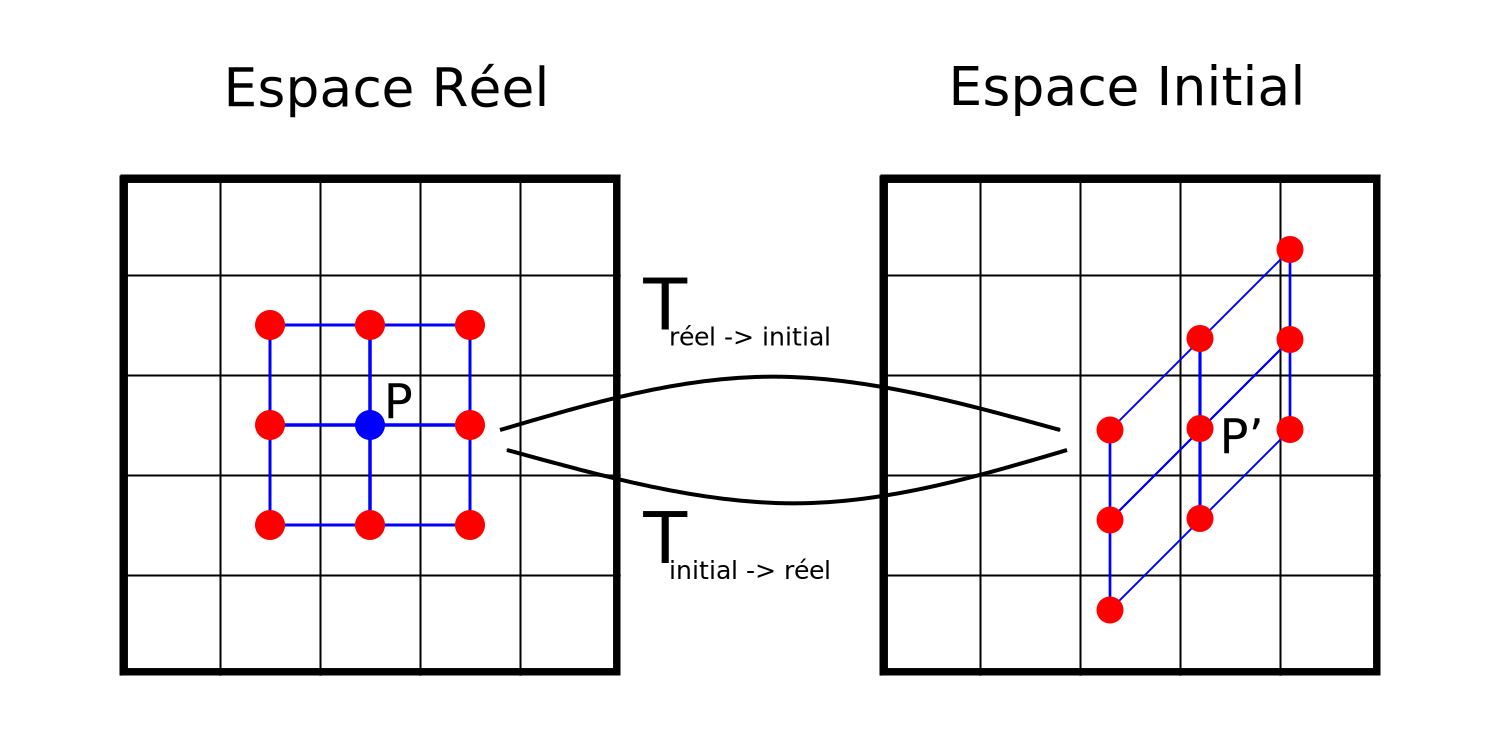
\includegraphics[width=.9\linewidth]{img/tetmesh_representation.png}
                \caption{Une illustration graphique du problème d'interpolation lors du passage en espace initial. Afin de trouver $f(P)$, il nous faut déterminer $f(P')$, qui nécessite une interpolation avec l'image de ses plus proches voisins dans l'espace initial, afin d'estimer correctement la valeur à lui attribuer.}
                \label{img:coordinate_change_interpolation_neighbor}
            \end{figure}

            Choisir le bon type d'interpolation n'est pas trivial. Tout d'abord, il requiert de savoir le type d'images donné en entrée. Nous ne possédons que des images non segmentées, nous pouvons donc appliquer tous les types d'interpolation explorés en section \ref{subsection:interpolation}. Si par la suite, le besoin se fait ressentir de segmenter les images avant leur reconstruction, nous avons fait en sorte d'avoir une implémentation reconfigurable, acceptant plusieurs méthodes d'interpolation différentes, et permettant l'ajout de nouvelle méthodes d'interpolation sans avoir besoin de changer la base de code présente.

            Comme on peut le voir dans la figure \ref{img:resampling}, le choix du type d'interpolation aura des conséquences différentes sur notre calcul de la valeur au point $P$. Une fois le bon type d'interpolation choisie pour l'opération à réaliser, il nous faut calculer la valeur au point $P'$ image de $P$ en espace initial, en prenant en compte du voisinage direct de $P$ dans l'espace réel. Nous évaluons ce voisinage comme l'ensemble des voxels de la grille partageant une primitive (face, arête, sommet) avec le voxel $V$ contenant le point $P$. Ce voisinage est la distance $L_\infty$. Ainsi, nous possédons un ensemble des voisins directs de $P$, afin de faire une estimation de sa valeur grâce à une méthode d'interpolation comme celles vues en section \ref{subsection:interpolation}.

            La dernière étape est la fusion des données des piles de coupes. En effet, pour tout point $P$, on peut calculer ses coordonnées dans l'espace de la pile de coupes 1, ou de la pile de coupes 2. Ainsi, il nous faut posséder une méthode pour comparer, analyser et attribuer les valeurs extraites du voisinage des points dans la pile 1 et dans la pile 2. Pour l'instant, nous faisons une moyenne des deux valeurs obtenues dans les deux jeux de données. Le code responsable pour l'interpolation est assez flexible pour supporter n'importe quel type d'opération que l'on voudrait appliquer. Par exemple, si par la suite nous souhaitons effectuer une opération plus complexe, nous n'aurions qu'à changer la fonction responsable de la fusion des valeurs obtenues dans les piles d'images. Plus d'informations seront disponibles sur l'implémentation de cette recherche dans la section \ref{section:implementation}.
		}
		% }}}

        Nous possédons donc une méthode robuste, permettant d'obtenir, à la volée, la valeur d'un point $P$ depuis les valeurs de ses voisins en espace initial. Cette méthode est efficace, précise, et ne demande pas d'autre information que la transformation, qui peut être dérivée des paramètres du microscope. Ainsi, nous pouvons effectuer cette méthode de recherche des voisins interactivement, afin de pouvoir reconstruire une grille de voxels en espace réel.
	}
    % }}}
    
    % generation de grille {{{
	\section{Génération de grille}\label{section:grid_generation}
	{
	    \iffalse
		\commentaire{buts de la section :~\begin{itemize}
		    \item présenter le besoin de re-générer des grilles
		    \item définir le coeur du problème
		    \item mettre en valeur par rapport aux méthodes de Tulane qu'est ce que ca peut nous apporter.
		    \item montrer l'avantage d'une méthode 'personnalisée' à ce problème
		    \item vu que c'est pas encore totalement fini, ne pas mettre de résultats, mais plutot montrer techniquement ce que ca peut théoriquement apporter
		\end{itemize}}
		\fi

		Passons maintenant à la génération de grille de voxels. En effet, afin de reconstruire l'échantillon analysé de manière exacte, il nous faut tout d'abord posséder une structure de données permettant une exploration rapide et simple d'un point, afin d'en étudier la topologie par la suite. Cette reconstruction de l'échantillon pourra également être utilisée par la suite dans une visualisation de l'échantillon acquis, via les méthodes vues en sections \ref{section:visualisation:cuttingplanes} et \ref{section:visualisation:subdomains}, ou encore via une méthode de visualisation multi-échelle. Si l'on souhaite afficher l'échantillon à plusieurs résolutions et donc à plusieurs niveaux de détail, il nous faut pouvoir générer des grilles de résolution et de taille arbitraires.

		Ainsi, nous devons créer une méthode permettant de générer une grille de voxels représentant l'échantillon, depuis les données présentes dans les différentes piles de coupes. Cette méthode doit pouvoir permettre de générer des grilles de taille et de résolution arbitraires, afin de permettre l'ajout d'une visualisation multi-résolution dans de futurs travaux. Grâce à nos travaux effectués en section \ref{section:voisins}, nous pouvons aisément passer d'un espace à un autre grâce à deux simples transformations par pile. En utilisant ces transformations, nous pouvons définir une structure de voisinage en un point $P$ notée $\mathcal{N}(P)$, permettant d'estimer la valeur que celui ci devrait prendre selon les valeurs aux points définis par $\mathcal{N}(P)$ dans les espaces propres aux piles de coupes. Cette méthode permet de générer des grilles à la volée, afin de ne pas dépendre de la taille de l'échantillon et de générer des grilles au besoin de l'utilisateur. Une représentation simplifiée de l'algorithme de génération de grille est disponible ci-après en \ref{algo:grid_gen}.

		\begin{algorithm}[h]
            \SetKwInOut{Input}{input}
            \SetKwInOut{Output}{output}
		    \Input{Un ensemble de $n$ piles d'images $S_0$, \ldots, $S_n$, une grille de voxels à générer $G$}
		    \Output{la grille de voxels $G$, générée}
            \ForAll{voxel $V$ de $G$}{
                Récupérer la position monde $P$ du centre de $V$\;
                Récupérer les positions des voisins $\mathcal{N}(P)$\;
                \ForAll{piles d'images $S$}{
                    Transformer $P$ en $P'$, avec $T_{\text{réel}\rightarrow\text{initial}}$ de $S$\;
                    \uIf{$P\prime~\in$ boite englobante de $S$}{
                        Transformer tous les points de $\mathcal{N}(P)$ en $\mathcal{N}'(P')$ avec $T_{\text{réel}\rightarrow\text{initial}}$ de $S$
                        Évaluer les valeurs de $\mathcal{N}'(P')$\;
                        Interpoler les valeurs de $\mathcal{N}'(P')$ trouvées selon le choix de l'utilisateur
                    }
                }
                Mélanger les valeurs obtenues selon un critère défini par l'utilisateur\;
                Attribuer cette valeur au voxel $V$\;
            }
            \captionsetup{width=.8\linewidth}
            \caption{Algorithme de génération de grilles, simplifié.}
            \label{algo:grid_gen}
		\end{algorithm}

		Afin de permettre de mieux estimer la valeur du point $P$ pour tout voxel, l'évaluation du voisinage s'effectue dans l'espace initial. Nous souhaitons conserver les variations du tissu de  l'échantillon présentes dans les captures afin de ne pas dévier de la vérité terrain donnée par le microscope. Cet algorithme, tel qu'il est conçu bénéficierait grandement d'une implémentation en parallèle, utilisant plusieurs coeurs afin de générer une grille plus rapidement. Toutefois, dû à la durée du stage nous n'avons pas pu explorer les gains de performances qu'offriraient une telle implémentation.
	}
	% }}}

	% implementation {{{
	\section{Implémentation}\label{section:implementation}
	{
	    % Plan section {{{
	    \iffalse
	    \commentaire{Travail effectué :~\begin{itemize}
	        \item structure de stockage d'image : permet transformations car elle contient matrice définissant world $\rightarrow$ object
	        \item structure de voisinage avec maillage tétraédrique construit dessus~\begin{itemize}
	            \item permet d'interpoler selon plusieurs métriques
	            \item permet d'interpoler avec barycentrique (grâce maillage)
	            \item permet de voyager dans le volume, et de demander une interpolation (fonctions implémentées ici)
	        \end{itemize}
	        \item visualisateur double-vue~\begin{itemize}
	            \item création scene
	            \item stockage imagestorage et tetmesh, permet de dessiner selon modalités données (real space or not)
	            \item shaders, et implémentation
	            \item color palette sur les images
	        \end{itemize}
        \end{itemize}
        }
        \fi
        % }}}

        % intro section implémentation {{{
        Le code source développé pendant ce stage sera publiquement disponible sur Gitlab peu après le rendu de ce rapport. Cliquez \href{https://www.gitlab.com/thibaulltt/visualisation}{ici}\footnote{\url{https://www.gitlab.com/thibaulltt/visualisation}} pour y accéder. La page d'accueil contiendra une explication de la structure du projet.
        
         Pour toutes les représentations de points, ou de vecteurs directionels, un vecteur à quatre dimensions fut utilisé. Ce choix fut effectué pour deux raisons : tout d'abord, les matrices de transformations d'un espace à un autre peuvent donc contenir un décalage originel $v_0$ comme expliqué en fin de section \ref{subsection:espaces_transfo}. De plus, OpenGL fonctionne uniquement avec des points à quatre dimensions, car le processus de rastérisation nécessite la projection de points dans un espace tridimensionnel afin de traiter les primitives géométriques en entrée. Toutefois, tous nos calculs se déroulent en espace tridimensionnel \og{}traditionnel~\fg, la dimension rajoutée à chacun des points est uniquement présente pour OpenGL, et n'affecte en aucun cas nos calculs.
	    
        L'implémentation des travaux effectués pendant ce stage fut effectuée par étapes. Tout d'abord, nous avons mis en place une méthode de chargement d'images, que nous avons ensuite testée par l'établissement d'une méthode d'exploration du volume par plans de coupe. Ensuite, une fois que ces travaux préliminaires visant à nous familiariser avec les jeux de données furent effectués, nous avons développé un "double visualisateur" de piles de coupes, permettant de voir ladite pile en espace initial ainsi qu'en espace réel, afin de pouvoir visualiser les effets de la reconstruction sur la pile d'images sur des exemples de petite taille. En même temps, nous avons implémenté une classe de grilles de voxels générique, permettant aussi bien le chargement d'images tridimensionnelles depuis le disque que la génération à la volée de grilles volumiques directement dans le programme. Ensuite, la méthode de recherche de voisins décrite en section \ref{section:voisins} fut implémentée de façon à pouvoir générer des grilles à la volée. Ainsi, à la fin de ce chapitre, nous comparerons le temps pris par notre travail sur la génération d'une grille de voxels par rapport aux résultats obtenus par Tulane en utilisant leur méthode de reconstruction de l'échantillon.
	    
        Durant l'implémentation de ces travaux, un des principaux buts était d'écrire une méthode de génération de grilles paramétrisable et extensible afin de pouvoir appliquer cette méthode à plusieurs cas d'utilisation, où bien à s'adapter à des changements dans la méthode d'acquisition du microscope. Ainsi, la majorité de nos classes seront soit génériques, permettant d'introduire facilement un nouveau comportement (lire un nouveau type de fichiers par exemple), ou bien paramétrisables afin de modifier les étapes effectuées lors du traitement des données (modifier les critères d'interpolation pour la génération de grille par exemple).
        % }}}

        % chargement & mémoire {{{
        \subsection{Chargement, écriture et gestion mémoire}
        {
            La première étape réalisé durant ce stage fut l'implémentation d'un lecteur d'image tridimensionnelle, afin de charger les jeux de données à reconstruire. Plusieurs itérations furent nécessaires afin d'arriver à l'architecture que nous proposons maintenant. Nous souhaitions avoir une méthode de chargement d'images tridimensionnelles rapide, permettant de gérer plusieurs formats d'images ou de grilles, et permettant une interface simple à utiliser, au cas où des collaborateurs de Tulane souhaiteraient étendre notre projet à différents cas d'utilisation.
	        
            Ainsi, nous avons implémenté une classe de lecteur de grilles/images tridimensionnelles générique appelé \texttt{GenericGridReader}, que nous avons spécialisé pour deux types de fichiers : \texttt{TIFF} et \texttt{DIM/IMA} (tous deux vus en section \ref{section:loading}). En effet, le fait de posséder une classe générique permet facilement d'étendre le processus de lecture depuis le disque à d'autres types de fichiers par la suite, en spécialisant la classe de base. Cette architecture fut également étendue aux classes responsables pour l'écriture de fichiers. Ainsi, lorsqu'une grille est générée, il nous est possible d'écrire ses fichiers en format \texttt{TIFF}, ou bien en \texttt{DIM/IMA}.
	        
            C'est également ici que nous pouvons charger des images à une résolution inférieure à leur résolution initiale. Pour l'instant, nous avons implémenté un simple re-échantillonnage au plus proche voisin à $\frac{1}{4}$ de la résolution initiale pour chacune des images. Toutefois, nous avons créé une architecture assez modulaire pour permettre d'autres types de re-échantillonage, qui pourront être implémentés par la suite.
	        
            Afin d'optimiser l'utilisation mémoire sur des stations de travail qui pourraient posséder peu de mémoire vive, les données chargées ne sont gardées que lors de la vie de l'objet responsable pour leur lecture, ou bien jusqu'à ce qu'une structure de grille de voxels ne requière les données pour sa propre utilisation.
            
            C'est également pendant le chargement que plusieurs données nécessaires à la grille de voxels sont chargés ou générés. Par exemple, lors du chargement de l'image en mémoire, une boite englobante des données est calculée: seules les valeurs supérieures à $\lambda=5$ sont conservées, le reste étant considéré comme du bruit. Ce seuil $\lambda$ est bien sur modifiable, et peut être mis à jour avec une autre valeur lors de l'exécution du programme.
        }
        % }}}

        % représentation grilles {{{
        \subsection{Représentation des données}
        {
            Afin de représenter les images tridimensionnelles issues du capteur, ainsi que les grilles de voxels à générer il nous faut posséder une structure de grille de voxels. Cette structure doit être assez générique pour permettre de représenter aussi bien les images 3D stockées sur disque en entrée que les grilles de voxels à générer en sortie. Elle doit aussi permettre de définir une grille dans un espace transformé quelconque. Nous avons donc implémenté une classe nommée \texttt{DiscreteGrid}, permettant de stocker une grille de voxels dans un espace transformé.

            Grâce à cette classe, nous pouvons tout aussi bien stocker les images 3D en entrée ainsi que les images 3D générées par notre programme. Cette classe contient quelques attributs utiles pour le traitement des données qui sont tous définis dans l'espace initial, et donc relatifs à la grille en elle même. Nous pouvons noter la présence d'attributs tels que la résolution de la grille en nombre de voxels, la taille des voxels de la grille (définie sans unités pour permettre une plus grande adaptation à d'autres images par la suite), ainsi que deux boites englobantes : une pour la grille en elle-même, ainsi qu'une boite englobante pour les données significatives (supérieures au seuil $\lambda$  défini par l'utilisateur). La boite englobante de la grille sert non seulement à définir la taille des voxels en fonction de la résolution de la grille, mais également à définir l'origine de la grille dans son espace initial ce qui est utile pour les grilles générées, qui peuvent ne pas se trouver à l'origine de l'espace réel. Nous possédons également une matrice de transformation $T_{\text{réel}~\rightarrow~\text{initial}}$ permettant de passer de l'espace réel à l'espace initial, ainsi que son inverse : $T_{\text{initial}~\rightarrow~\text{réel}}$. Toutefois, étant donné la complexité du calcul de l'inverse d'une matrice, celle-ci est pré-calculée lorsqu'une matrice $T_{\text{réel}~\rightarrow~\text{initial}}$ est définie pour la grille.

            \begin{figure}[h]
                \centering
                \includegraphics[width=.8\linewidth]{img/grid_properties_initial_space.png}
                \captionsetup{width=.8\linewidth}
                \caption{Une représentation simplifiée en 2D de quelques une des propriétés de la grille, dans son espace initial. En (a), la boîte englobante de la grille de voxels. En (b), la boîte englobante des données de cette grille. En (c), les dimensions d'un voxel dans la grille. En (d), les données considérées comme significatives dans cette grille. En (e), la résolution de la grille de voxels.}
                \label{img:grid_properties_initial_space}
            \end{figure}

            Lors du chargement d'une image 3D issue d'une acquisition faite par le microscope, les données brutes sont chargées en mémoire en même temps que les caractéristiques de l'image en elle-même. Une fois ce chargement effectué, il n'est plus possible de modifier les caractéristiques intrinsèques à la grille de voxels. Les seules caractéristiques pouvant changer sont les paramètres de la transformation $T_{\text{réel}~\rightarrow~\text{initial}}$ associée à la pile d'images. Dans son espace initial, la grille est représentée comme décrit en section \ref{section:memory}, où chaque voxel est un voxel unitaire (de côté 1) afin d'obtenir un temps d'accès mémoire constant pour les données relatives à la grille. La position ainsi que la forme que la grille est censée avoir en espace réel est ainsi entièrement définie par la transformation qui lui est associée.

            Avant la génération des données d'une grille de voxels considérée comme "de sortie", il nous est possible de tout modifier : la résolution de cette grille de voxels, sa boite englobante ainsi que la dimension de ses voxels. Ainsi, une fois que les données en entrée sont chargées, nous pouvons générer une boite englobante optimisée selon les données afin de reconstruire l'échantillon efficacement. À partir de cette boite englobante ainsi que d'une résolution de grille, il nous suffira de calculer les positions des voxels de la grille de sortie puis d'itérer sur celles-ci afin d'appliquer des méthodes d'interpolation sur les voisins dans les espaces initiaux aux piles d'images. Ainsi, nous pourrons déterminer les valeurs à donner à chacun des voxels de la grille de sortie.
	        
            Dans un premier temps, cette génération de grilles de sortie prend entièrement place en mémoire, avec des jeux de données chargés intégralement en mémoire. Toutefois, il est aisé de changer ce comportement afin de générer des grilles en mode \og{}hors-ligne~\fg, sans avoir besoin de charger les données des grilles d'entrée en mémoire, ce qui permet de s'affranchir d'une des principales contraintes dans ce processus de reconstruction. Si le format de fichier possède une structure de grille connue, comme par exemple pour les fichiers \texttt{DIM/IMA} comme vu en section \ref{section:loading} alors il est possible de ne jamais avoir besoin de charger le fichier afin d'effectuer des opérations dessus. Ainsi, il est donc possible de reconstruire des grilles de plusieurs centaines de gigaoctets sur un ordinateur ne possédant que peu de mémoire vive, au coût d'une augmentation de temps considérable dû à la latence de lecture des données depuis un disque dur. Une comparaison schématique des deux méthodes est disponible en figure \ref{img:grid_gen}. %Malheureusement, dû à des retards engendrés dûs à des problèmes personnels pendant le confinement, cette partie de génération de grille n'a pas pu être finie à temps.

            \begin{figure}[h]
                \centering
                \begin{subfigure}{.8\linewidth}
                    \centering
                    \includegraphics[width=\linewidth]{img/grid_gen_method_online.png}
                    \captionsetup{width=\linewidth}
                    \caption{Méthode de génération de grilles "en ligne" : les données sont intégralement chargées en mémoire (d'un coup ou par morceaux), pour générer la grille, qui est ensuite écrite sur le disque.}
                    \label{img:grid_gen:online}
                \end{subfigure}
                \begin{subfigure}{.8\linewidth}
                    \centering
                    \includegraphics[width=\linewidth]{img/grid_gen_method_offline.png}
                    \captionsetup{width=\linewidth}
                    \caption{Méthode de génération de grilles "hors-ligne" : le jeu de données n'est jamais chargé directement en mémoire pour générer la grille. Les seules données lues sont les données nécessaires à la génération d'une donnée pour un voxel de la grille de sortie, qui est ensuite écrit directement sur disque.}
                    \label{img:grid_gen:offline}
                \end{subfigure}
                \captionsetup{width=.8\linewidth}
                \caption{Comparaison des deux méthodes de génération de grilles : en ligne, et hors-ligne}
                \label{img:grid_gen}
            \end{figure}
        }
        % }}}

        % voisinnage {{{
        \subsection{Structure de voisinage et génération de grilles}
        {
            La structure de voisinage permet pour tout point $P$ dans une grille $\mathcal{G}$ de générer un maillage permettant de simuler les positions du voisinage direct de $P$, noté $\mathcal{N}(P)$. Ce voisinage est mobile, et permet donc d'analyser les valeurs de n'importe quel voxel dans une grille. En effet, comme vu en section \ref{section:grid_generation} nous avons besoin de pouvoir déterminer les valeurs de ces points dans les espaces initiaux aux images volumiques en entrée.

            En plus de stocker les informations du voisinage $\mathcal{N}(P)$, cette structure possède également quelques pointeurs permettant de définir de multiples grilles volumiques en entrée, ainsi qu'une unique grille à générer. Ainsi, cette structure est également responsable du déroulement de l'algorithme de génération de grille. En effet, étant donné que cette structure de voisinage permet de donner les positions des voisins directs à un point $P$ dans l'espace initial de la grille à générer, il est naturel de pouvoir redéfinir ces points dans un espace secondaire grâce à une matrice de transformation d'une des grilles en entrée.

            Comme vu en section \ref{section:grid_generation}, nous appliquons l'algorithme de génération de grilles à chacun des voxels de la grille à générer, afin de pouvoir obtenir les valeurs de ses voisins dans les différents espaces initiaux des différentes piles d'image en entrée. L'algorithme choisi pour l'interpolation est défini par l'utilisateur par une liste disponible sur l'interface utilisateur créée avec \textit{Qt}. Une fois les données de plusieurs grilles obtenues, elles sont fusionnées avec une simple moyenne pour l'instant. Toutefois, cette partie pourra être modifiée par la suite, afin de permettre à d'autres méthodes de fusion d'être implémentées.
        }
        % }}}

        % visualisation {{{
        \subsection{Visualisation du jeu de données}
        {
            Afin de pouvoir visualiser nos jeux de données, il nous a fallu implémenter un visualisateur d'image médicale. Grâce à l'utilisation de \textit{Qt}, d'\textit{OpenGL} ainsi que de \textit{libQGLViewer}, cette tâche fut grandement simplifiée. La création de fenêtres, la gestion des processeurs graphiques pour l'affichage ainsi que du clavier/souris pour l'entrée utilisateur furent pris en charge par ces bibliothèques et APIs.

            Nous avons donc commencé par créer un premier visualisateur simple, permettant de visualiser uniquement les données chargées en mémoire comme vu en figure \ref{img:cubes}. Comme expliqué en section \ref{section:visualisation:cuttingplanes}, nous devons d'abord charger les images depuis le disque, puis les envoyer sur la mémoire du processeur graphique grâce aux fonctions offertes par \textit{OpenGL}. Ensuite, nous envoyons sur ce même processeur graphique des points, arrangés de façon à former un cube. En plus d'envoyer ces points, nous donnons au processeur graphique une coordonnée de texture par sommet, afin que celui-ci puisse afficher l'image tridimensionnelle chargée auparavant sur les bonnes faces du cube. Ce visualisateur fut développé au début du stage, afin de vérifier que le chargement des données s'effectuait correctement, et fut amélioré itérativement au cours du développement du projet.

            L'une des premières modifications apportées à ce visualisateur simple fut l'ajout d'une échelle de couleurs sur l'affichage de l'image médicale. En effet, l'oeil humain discerne mieux les différences de couleurs que celles de niveaux de gris. Cette échelle de couleur ne fut appliqué qu'au moment de l'affichage, et ne nécessite aucune modification des données en entrée. Comme cela est décrit dans l'annexe technique, le processus d'affichage d'un élément tridimensionnel à l'aide d'\textit{OpenGL} produit pour chacun des pixels de l'écran un ensemble de fragments, des échantillons d'une primitive géométrique parmi celles affichées contenant les informations nécessaires pour déterminer une couleur que prendra ce pixel à la fin de l'opération d'affichage. Ainsi, au lieu d'afficher la nuance de gris de l'image directement, elle est d'abord utilisée afin de déterminer une couleur en espace HSV~\cite{cite_hsv_original_paper}. Ensuite, cette couleur HSV est convertie en espace RGB afin de donner une couleur finale au fragment. Le résultat est visible en figure \ref{img:visualisateur:color_scale_comparaison}.

            \begin{figure}[h]
                \centering
                \begin{subfigure}{.45\linewidth}
                    \centering
                    \includegraphics[width=.9\linewidth]{img/visu_screens/black_white.jpg}
                    \captionsetup{width=.9\linewidth}
                    \caption{Les données brutes, en niveaux de gris.}
                    \label{img:visualisateur:color_scale_comparaison:black_white}
                \end{subfigure}
                \begin{subfigure}{.45\linewidth}
                    \centering
                    \includegraphics[width=.9\linewidth]{img/visu_screens/colored.jpg}
                    \captionsetup{width=.9\linewidth}
                    \caption{Une échelle de couleurs appliquée.}
                    \label{img:visualisateur:color_scale_comparaison:colored}
                \end{subfigure}
                \captionsetup{width=.8\linewidth}
                \caption{Une comparaison entre l'affichage des données brutes et l'application d'une échelle de couleurs.}
                \label{img:visualisateur:color_scale_comparaison}
            \end{figure}

            En plus de l'affichage de cette échelle de couleurs, nous avons ajouté la possibilité de définir une plage de valeurs à afficher avec cette échelle de couleurs, afin de pouvoir facilement discerner les différentes plages de valeurs sur un plan affiché. Ainsi, les valeurs de gris situées au dessus d'une borne supérieure seront affichés en blanc, tandis que les valeurs en dessous d'une borne inférieure seront affichées en noir. Une visualisation de cette fonctionnalité est disponible en figure \ref{img:visualisateur:functions:thresholds}. De plus, étant donné le faible contraste entre les côtés du cube, et à des fins de débogage, un affichage des arêtes en une passe de dessin fut implémentée. Son implémentation fut largement adaptée depuis \cite{cite_wireframe}, adaptée et simplifiée à notre cas d'utilisation. Cela permet de voir les délimitations des faces composant un maillage plus précisément. Une illustration est donnée en figure \ref{img:visualisateur:functions:wireframe}.

            \begin{figure}[h]
                \centering
                \begin{subfigure}{.45\linewidth}
                    \centering
                    \includegraphics[width=.9\linewidth]{img/visu_screens/thresholds.jpg}
                    \captionsetup{width=.9\linewidth}
                    \caption{L'image médicale, avec l'échelle de couleurs appliquée uniquement aux valeurs de gris supérieures à 5.}
                    \label{img:visualisateur:functions:thresholds}
                \end{subfigure}
                \begin{subfigure}{.45\linewidth}
                    \centering
                    \includegraphics[width=.9\linewidth]{img/visu_screens/wireframe.jpg}
                    \captionsetup{width=.9\linewidth}
                    \caption{Une visualisation des arêtes composant le cube sur lequel est appliqué l'image tridimensionnelle.}
                    \label{img:visualisateur:functions:wireframe}
                \end{subfigure}
                \captionsetup{width=.8\linewidth}
                \caption{Quelques fonctionnalités supplémentaires du visualisateur d'images médicales.}
                \label{img:visualisateur:functions}
            \end{figure}

            Au moment où l'algorithme de génération de grilles commença à être implémenté, nous avions besoin de visualiser les deux espaces possibles pour une pile d'image simultanément, afin de vérifier visuellement que les transformations d'un espace à un autre s'effectuaient correctement. Ainsi, nous avons implémenté un visualisateur permettant de visualiser les piles d'images en espace réel ainsi que dans leurs espaces initiaux respectifs. Pour cela, nous avons implémenté une classe de scène, permettant de regrouper les données à afficher en un seul endroit, afin de ne pas dupliquer d'informations. Cette scène est ensuite affichée sur plusieurs fenêtres de \texttt{libQGLViewer}, afin que l'on puisse interagir avec cette scène grâce au clavier et à la souris. Le processus de mise en place est similaire au visualisateur d'avant, mais permet plus de flexibilité, dû au fait que l'on puisse l'afficher les données chargées en plusieurs espaces à la fois grâce à l'utilisation de \textit{shaders}\definition{Fichier de code permettant de programmer une partie du processus de traitement de la géométrie par \textit{OpenGL}}. Une illustration est disponible en figure \ref{img:visualisateur:double}.

            \begin{figure}[h]
                \centering
                \includegraphics[width=.9\linewidth]{img/visu_screens/double_view_01.jpg}
                \captionsetup{width=.9\linewidth}
                \caption{Le double visualisateur de pile d'images. À gauche, la pile d'image en espace réel. À droite, la pile d'images dans son espace initial.}
                \label{img:visualisateur:double}
            \end{figure}

            Ces visualisateur permettent d'afficher plusieurs grilles afin de visualiser leur position dans l'espace réel, ce qui permet de vérifier visuellement si les données sont bien transformées avant de générer une grille de données. Ainsi, en figure \ref{img:visualisateur:grids} on peut voir la grille de voxels à générer affichée avant et après sa génération (la taille de la grille fut exagérée pour des raisons de démonstration).

            \begin{figure}[h]
                \centering
                \begin{subfigure}{.45\linewidth}
                    \centering
                    \includegraphics[width=.9\linewidth]{img/visu_screens/grid_empty.jpg}
                    \captionsetup{width=.8\linewidth}
                    \caption{Une grille de voxels, prévisualisée avant d'être générée.}
                    \label{img:visualisateur:grids:empty}
                \end{subfigure}
                \begin{subfigure}{.45\linewidth}
                    \centering
                    \includegraphics[width=.9\linewidth]{img/visu_screens/grid_generated.jpg}
                    \captionsetup{width=.8\linewidth}
                    \caption{La même grille de voxels, générée et affichée.}
                    \label{img:visualisateur:grids:generated}
                \end{subfigure}
                \captionsetup{width=.9\linewidth}
                \caption{Un affichage de plusieurs grilles de voxels de types différents. La grille en gris à gauche est une grille à générer, tandis que la grille déjà contruite derrière est une pile d'images issue du microscope de Tulane.}
                \label{img:visualisateur:grids}
            \end{figure}

            Les visualisateurs développés pendant ce stage permettent l'établissement d'une base de code facile à prendre en main afin d'ajouter des modalités de visualisations plus compliquées. Grâce à l'utilisation de \textit{shaders} pour le visualisateur double, nous avons pu développer une méthode d'affichage adaptée à nos besoins actuels, et pouvant s'adapter à nos besoins futurs.
        }
        % }}}

        % résultats {{{
        \subsection{Résultats}
        {
            Maintenant que nous possédons un algorithme de génération de grille, il est temps de comparer cette méthode à celle mise en place à Tulane. Ainsi, nous allons mettre en place un banc de test permettant de déterminer les performances de notre méthode. En plus du banc de test, nous pouvons vérifier visuellement que la méthode de génération de grille fonctionne correctement grâce au visualisateur double.

            Nos collaborateurs à Tulane nous ont fait parvenir un échantillon de leurs temps de calcul pour reconstruire une acquisition avec leur méthode. Nous pouvons ainsi établir un protocole de test afin d'obtenir des résultats en cohésion avec les leurs. Nous avons donc choisi de faire deux séries de tests. Chacune reconstruira l'échantillon en entrée avec une résolution de $1024~\times~1024~\times~1000$, en chargeant 1000 images en entrée. La différence sera dans la méthode d'interpolation utilisée pour générer la grille. En effet, une série de tests s'effectuera en utilisant une interpolation au plus proche voisin, et une série de tests s'effectuera avec de l'interpolation trilinéaire. 

            Les tests furent effectués sur un ordinateur portable, équipé d'un \textit{Intel Core i7 9750H} (6 c\oe{}urs tournant jusqu'à 4.9GHz) ainsi que 16 gigaoctets de RAM. Tandis que Tulane étaient équipés d'un \textit{Intel Xeon Processor E5-2699} (18 c\oe{}urs tournant jusqu'à 3.6GHz), avec 128 gigaoctets de RAM. Les résultats furent moyennés sur 10 mesures pour chacun des cas de tests. Tout d'abord, voici les temps que nous pouvons obtenir grâce à notre méthode pour la reconstruction d'une pile de 1000 images :\bigskip

            {
                \centering
                \begin{tabular}{|c|c|c|}
                    \hline
                    \textbf{ } & \textbf{Plus proche voisin} & \textbf{Trilinéaire} \\ \hline %  & \textbf{Résultats Tulane}
                    \textbf{Temps} (s) & 30.82s & 196.38s \\ \hline
                    \textbf{Vitesse} (gigavoxel/heure) & 122.5 GV/h & 19.2 GV/h \\
                    \hline
                \end{tabular}
            }\bigskip
            
            Toutefois, les résultats que Tulane nous ont fait parvenir sont des résultats pour la génération d'une grille depuis 10 piles de coupes. Ainsi, afin d'obtenir une estimation du temps que cela prendrait, il nous suffit de multiplier par 10 afin de comparer nos résultats :\bigskip

            {
                \centering
                \begin{tabular}{|c|c|c|c|}
                    \hline
                    \textbf{ } & \textbf{Plus proche voisin} & \textbf{Trilinéaire} & \textbf{Résultats Tulane} \\ \hline %  
                    \textbf{Temps} (s) & 308.2ss & 1963.8s & 4610.5s \\ \hline
                    \textbf{Vitesse} (gigavoxel/heure) & 122.5 GV/h & 19.2 GV/h & 11,9 GV/h \\
                    \hline
                \end{tabular}
            }\bigskip

            Nous sommes donc deux fois plus rapide que Tulane pour générer un échantillon de prostate à partir de piles d'images de leur microscope, en utilisant une interpolation trilinéaire, et jusqu'à 10 fois plus rapide en utilisant l'interpolation au plus proche voisin. Toutefois, il reste à vérifier si l'interpolation est correcte visuellement. Pour cela, tournons nous vers un échantillon de reconstruction, en figure \ref{img:results}.

            \begin{figure}[h]
                \centering
                \begin{subfigure}{.5\linewidth}
                    \centering
                    \includegraphics[width=.9\linewidth]{img/results/original.png}
                    \captionsetup{width=.9\linewidth}
                    \caption{L'échantillon de prostate, originellement.}
                    \label{img:results:original}
                \end{subfigure}
                \begin{subfigure}{.5\linewidth}
                    \centering
                    \includegraphics[width=.9\linewidth]{img/results/nearest.png}
                    \captionsetup{width=.9\linewidth}
                    \caption{Reconstruit avec méthode au plus proche voisin.}
                    \label{img:results:nearest}
                \end{subfigure}
                \begin{subfigure}{.5\linewidth}
                    \centering
                    \includegraphics[width=.9\linewidth]{img/results/trilinear.png}
                    \captionsetup{width=.9\linewidth}
                    \caption{Reconstruit avec méthode trilinéaire.}
                    \label{img:results:trlinear}
                \end{subfigure}
                \captionsetup{width=.9\linewidth}
                \caption{Une vue de proximité de l'échantillon reconstruit.}
                \label{img:results}
            \end{figure}
            
            Nous pouvons voir que l'interpolation au plus proche voisin donne une bonne estimation de l'échantillon en espace réel, mais ne permet pas de lisser les micro-variations présentes dans le tissu. Toutefois, l'interpolation trilinéaire permet d'uniformiser le contenu de l'acquisition lors de la reconstruction. Ainsi, grâce aux méthodes décrites en section \ref{section:visualisation:cuttingplanes} et \ref{section:visualisation:subdomains}, nous pouvons également visualiser cet échantillon reconstruit en trois dimensions (figure \ref{img:reconstruction:volumic}).
            
            \begin{figure}[h]
                \centering
                \begin{subfigure}{.48\linewidth}
                    \centering
                    \includegraphics[width=.9\linewidth]{img/results/3D/volumic_01.png}
                    \captionsetup{width=.8\linewidth}
                    \caption{Une représentation volumique de l'échantillon reconstruit.}
                    \label{img:reconstruction:volumic:01}
                \end{subfigure}
                \begin{subfigure}{.48\linewidth}
                    \centering
                    \includegraphics[width=.9\linewidth]{img/results/3D/volumic_02.png}
                    \captionsetup{width=.8\linewidth}
                    \caption{Une représentation volumique de l'échantillon reconstruit.}
                    \label{img:reconstruction:volumic:02}
                \end{subfigure}
                \captionsetup{width=.8\linewidth}
                \caption{Quelques captures d'écran obtenues avec la méthode de visualisation volumique décrite en \ref{section:visualisation:subdomains}}
                \label{img:reconstruction:volumic}
            \end{figure}
        }
        % }}}
    }
    % }}}
}

% VIM modeline : do not touch !
% vim: set spell spelllang=fr :


	% Chapitre 05 : travaux à venir / thèse / peut être conclusion
\chapter{Travaux à venir \& difficultés}



	% Chapter 5 : Conclusion, réflection & difficultés rencontrées, ouverture
\chapter{Conclusion}\label{chapter05:conclusion}
{
	\commentaire{
		\begin{enumerate}
			% conclusion {{{
			\item Conclusion : travaux effectués. Buts originaux :~\begin{itemize}
				\item Gestion de données massives [x] :\begin{itemize}
					\item on peut en effet charger des images massives en mémoire, même si celles ci sont moins massives que les données réelles de Tulane (travail à suivre après le stage)
					\item on peut aussi charger des versions basse résolution des images, au cas où les full-res ne rentrent pas en mémoire (option de downsampling dans le loader)
				\end{itemize}
				\item Exploration interactive [x] :~\begin{itemize}
					\item On peut utiliser des plans de coupe dans l'application en single-view, pour traverser le volume (plans de coupe surement ajoutés dans vue double sous peu, mais peut être après rapport/soutenance)
					\item Techniquement, on pourait aussi exporter une grille et le voir avec Texture3D
				\end{itemize}
				\item Visualisation multi-résolution~\begin{itemize}
					\item Ce but est plus flou, parce que oui, on peut générer des grilles à plusieurs résolutions et les voir, mais bon, ca casse le côté interactif de la visu ...
				\end{itemize}
			\end{itemize}
			% }}}
			% reflection {{{
			\item Réflection : difficultés encontrées\begin{itemize}
				\item confinement $\rightarrow$ pas de réunion en présentiel et tous les jours se ressemblent et s'assemblent $\rightarrow$ moral au plus bas
				\item exemple : opengl : je me suis pas posé et ai plutot foncé tête baissée $\rightarrow$ perte de temps, d'énergie et de toute envie de quoi que ce soit
				\item problème perso : ne veut pas faire de petits pas, mais plutot un grand en + de tps
				\item ouverture : + de travail sur moi même \& ma facon de travailler (malheureusement, seule ouverture possible dans ce contexte)
			\end{itemize}
			% }}}
			% futur, pour juillet & thèse {{{
			\item Ouverture : possibilités de continuation dans un futur proche\begin{itemize}
				\item En juillet\begin{enumerate}
					\item Implémenter version offline, sans accès graphique
					\item Implémenter version incrémentale et/ou partielle (d'abord recalage, sauvegardé dans un fichier, puis stitching des images en grille)
					\item Faire plutot visu multi res
					\item Et d'autres encore
				\end{enumerate}
			\item Ouverture : thèse ! Travaux à venir :\todo{A garder ?}\begin{enumerate}
					\item Remeshing des glandes pour démarrer le travail de reconstruction approfondie et détaillé (?)
					\item ???
				\end{enumerate}
			\end{itemize}
			% }}}
		\end{enumerate}
	}

	\section{Travail réalisé}
	{
		Durant ce stage, nous devions achever les trois objectifs suivants :~\begin{itemize}
			\item une méthode de gestion de données massives,
			\item une méthode d'exploration interactive de ces données,
			\item et une méthode de visualisation multi-résolution.
		\end{itemize}\par
		Nous avons pu en effet gérer les données massives venant du processus de capture développé par l'université de Tulane. Grâce à l'utilisation d'une simplification des images à la volée, nous pouvons confortablement charger une pile d'image entière en mémoire. De plus, nous avons présenté une méthode plus intelligente de chargement des données, qui permettrait de réduire l'empreinte mémoire de notre programme\todo{pour que plus de systèmes le fassent tourner, à mentionner ?}.\par
		Nous avons également présenté deux méthodes pour l'exploration interactive des données, une fois chargés en mémoire, avec deux cas d'utilisation différents. Ces deux méthodes nous permettent de visualiser interactivement les modèles selon le type de données en entrée, et le type d'observation à effectuer.\par
		Enfin, même si ces travaux s'achèveront au courant du mois de juillet, la vue en multi-résolution des données est possible car nous avons créé deux méthodes permettant d'analyser les données et d'en générer de nouvelles de résolution et tailles différentes, à la volée.\par
	}

	\section{Réflexion}
	{
		\commentaire{Cette partie est entièrement personnelle, donc utilisation naturelle de la première personne. À garder, ou réécrire en non-inclusif (qui rendrait cette partie non nécessaire) ? Si réécriture en non-personnel, uniquement parler des problèmes techniques, et laisser les explications personnelles pour la soutenance peut être ?}\par
		Il est impossible de parler des difficultés rencontrées pendant le stage sans parler de la période de confinement engagée par l'\'Etat Français. En effet, la mise en place d'une mesure de confinement à domicile a rendu beaucoup plus compliqué les réunions entre toutes les personnes dans le stage. La distanciation sociale ne fut pas que physique, elle fut aussi mentale, pesant lourd sur les résultats du stage et les travaux accomplis. Une des conséquences de cette distanciation fut accrue par un problème technique que j'ai rencontré, qui a mis beaucoup trop de temps à être réglé à cause de cette baisse de moral, qui entraîne un cercle vicieux.\par
		De plus, un de mes gros défauts personnels viennent d'un manque d'organisation : je n'arrive pas à découper les tâches en morceaux assez petits pour permettre une progression fluide des travaux de recherche. Je me retrouve uniquement coincé devant un immense mur de tâches monolithiques duquel je ne peux pas m'échapper. Et la distanciation, couplée à un très grand sentiment de monotonie pendant le confinement ont impacté fortement mes capacités à travailler efficacement pendant plus d'un mois.\par
		Mais tout n'est pas perdu. Le retour progressif à la normale va me forcer à reprendre un rythme plus soutenu, me forcer à reprendre l'habitude de montrer une amélioration plus souvent, et je vais bien entendu faire de mon possible pour toujours essayer de décomposer au plus les problèmes afin de ne plus me retrouver bloqué comme pendant cette période de confinement.
	}

	\section{Futurs travaux}
	{
		\wip{Changer : multi-échelle après, uniquement si temps : d'abord offline et incrémentale}\par
		Malgré les difficultés rencontrées, nous avons réussis à atteindre la majorité de nos objectifs au moment de l'écriture du rapport. Mais nous avons encore du travail à effectuer avant la fin du stage en fin juillet. Il nous reste bien sûr à finir les fonctionnalités en cours d'implémentation comme discuté auparavant : une possibilité de visualisation multi-échelle par génération de multiples grilles hiérarchiques, la possibilité d'effectuer le processus de reconstruction hors-ligne, afin de pouvoir s'affranchir de la visualisation et de permettre de faire fonctionner la reconstruction sur un serveur distant sans sortie vidéo.\par
		%
	}
}

% VIM modeline : do not touch !
% vim: set spell spelllang=fr :


\end{document}

% VIM modeline : do not touch !
% vim: set spell spelllang=fr :
